\documentclass[11pt, a4paper]{article}
% Set the fonts of the document
\usepackage{inconsolata} % Monospace font
\usepackage{helvet} % Sans-serif font
\usepackage[
    libertine, % do not override the sans-serif-font
    tt = false % do not override the monospace font
]{libertine} % Main font (serif)

\usepackage[
    top = 3cm,
    bottom = 3cm,
    left = 2.5cm,
    right = 2.5cm
]{geometry}

\usepackage[english]{babel}
\usepackage{xspace}
\usepackage{booktabs}
\usepackage{enumitem}
\usepackage[xcolor]{mdframed}
\usepackage{amsmath}
\usepackage{amssymb}
\usepackage{amsthm}
\usepackage{mathrsfs}
\usepackage{stmaryrd}
\usepackage{float}
\usepackage{listings}
\usepackage{parskip}
\usepackage[
    labelfont = {small, bf},
    textfont = {small}
]{caption}
\usepackage{subcaption}
\usepackage{circledsteps}
\usepackage{hyperref}

% ====================================================================

\newcommand{\eg}{e.g.,\xspace}
\newcommand{\ie}{i.e.\xspace}
\newcommand{\etal}{\textit{et~al.}\xspace}

\newcommand{\todo}[1]{{\centering\textbf{\textcolor{red}{[TODO : #1]}}\xspace}}

\newcommand{\vsc}{Visual Studio Code\xspace}

\DeclareRobustCommand{\iLaTeX}{\mbox{{{\itshape i}-\hspace{-0.25mm}}\LaTeX{}}}

% Document title
\newcommand{\makedoctitle}[1]{%
\begin{center}
    \color{black!75}
    {\Large{Longitudinal study of \iLaTeX}} \\
    \noindent\rule{12cm}{0.4pt} \\[1.5em]
    \color{black}
    {\Huge{#1}} \\[0.5em]
    % \noindent\rule{16cm}{0.4pt}
\end{center}
}

% Custom framed environments
\newmdenv[
    linecolor = red!50!black,
    backgroundcolor = red!2,
    skipabove = 1em,
    skipbelow = 1em,
    innertopmargin = 1em,
    innerbottommargin = 1em,
    frametitle = {Warning},
    frametitlebackgroundcolor = red!5,
    % startinnercode = \centering\bgroup,
    % endinnercode = \egroup
    nobreak = true
]{warning}

\newmdenv[
    linecolor = blue!50!black,
    backgroundcolor = blue!2,
    skipabove = 1em,
    skipbelow = 1em,
    innertopmargin = 1em,
    innerbottommargin = 1em,
    frametitle = {Good to know},
    frametitlebackgroundcolor = blue!5,
    % startinnercode = \centering\bgroup,
    % endinnercode = \egroup
    nobreak = true
]{info}

\newmdenv[
    linecolor = green!50!black,
    backgroundcolor = green!2,
    skipabove = 1em,
    skipbelow = 1em,
    innertopmargin = 1em,
    innerbottommargin = 1em,
    frametitle = {Example},
    frametitlebackgroundcolor = green!5,
    % startinnercode = \centering\bgroup,
    % endinnercode = \egroup,
    % nobreak = true
]{example}

% Style of code blocks
\lstdefinestyle{custom-latex}{
    language={[LaTeX]TeX},
    backgroundcolor=\color{white},
    commentstyle=\color{black!50},
    keywordstyle=\color{green!50!black},
    numberstyle=\tiny\color{red!50!black},
    stringstyle=\color{blue!50!black},
    basicstyle=\ttfamily\small,
    breakatwhitespace=false,         
    breaklines=true,
    keepspaces=true,
    numbers=none,
    tabsize=4,
    aboveskip={1em},
    belowskip={0.7em}
}

\lstdefinestyle{custom-latex-example}{
    language={[LaTeX]TeX},
    commentstyle=\color{black!50},
    keywordstyle=\color{green!50!black},
    numberstyle=\tiny\color{red!50!black},
    stringstyle=\color{blue!50!black},
    basicstyle=\ttfamily\footnotesize,
    breakatwhitespace=false,         
    breaklines=true,
    keepspaces=true,
    numbers=none,
    tabsize=4,
    aboveskip={1em},
    belowskip={-1ex}
}

% Description of a command/environment (for the cheat sheet)
\newcommand{\commanddesc}[1]{{\color{black!80}{#1}}}


% Command to produce a circled number to reference a step represented in a figure
\definecolor{FigStepColor}{HTML}{BC43F0}

\DeclareRobustCommand{\figstep}[1]{%
    \Circled[%
        inner color=white,%
        outer color=white,%
        fill color=FigStepColor%
    ]{\sffamily\textbf{#1}}%
}

% These two packages are required for iLaTeX to work!
\usepackage{ilatex}
\usepackage{gridlayout}

\begin{document}

\makedoctitle{Introduction to \iLaTeX{}}
\vfill
\tableofcontents
% \newpage


%%%%%%%%%%%%%%%%%%%%%%%%%%%%%%%% START OF CONTENT

\section{What is \iLaTeX{}?}
\iLaTeX{} is a research prototype of a new kind of editor for \LaTeX{} documents.
It is built on top of Visual Studio Code, an open-source code editor.
\iLaTeX{} looks and works like other \LaTeX{} editors such as TeXstudio and Overleaf, but it also offers a new kind of features we call \emph{interactive intermediate representations}---or IIR for short.

IIRs constitute an alternative way to visualise and manipulate certain parts of a \LaTeX{} document than the source code or the generated PDF.
Each IIR is bound to a piece of \emph{visualisable code}, \ie code that can be visualised through an IIR.
IIR are an optional feature of \iLaTeX{}: since the source code of your documents remains accessible at all times, you can also use \iLaTeX{} like a standard \LaTeX{} editor!



\section{\iLaTeX{} in this study}

This study is made of two successive parts that are independent from each other.
At some points in the study, you may be requested or forbidden to use IIRs by the investigator:
\begin{itemize}
    \item If you are \textbf{requested} to use IIRs, you should use IIR as much as possible to perform the task you have been assigned. However, if you believe you cannot accomplish what you want to do with an IIR, or if you think editing the code directly would be faster, you are still allowed to use the code editor.
    \item If you are \textbf{forbidden} to use IIRs, you must use \iLaTeX{} like a standard code editor (you can still use all the regular code editing features provided by Visual Studio Code such as search-and-replace and keyboard shortcuts);
    \item \textbf{Otherwise}, you are free to decide whether you want to use IIRs or not!
\end{itemize}

In case of doubt of whether you can or should use IIR for the current task, please ask the investigator.



\section{Usage of \iLaTeX{}}
In order to use an IIR, two steps are required:
\begin{enumerate}[noitemsep]
    \item the IIR must be \emph{created} from a piece of visualisable code by \iLaTeX{};
    \item the IIR must be \emph{displayed} by the user.
\end{enumerate}

Each step is explained in more details below.

\subsection{Creating an IIR}
\iLaTeX{} will automatically attempt to find all pieces of visualisable code in your document and to create an IIR for every of them.
Visualisable code is detected by the usage of special \LaTeX{} commands and environments that are known to be visualisable by \iLaTeX{}.
The detail of every command and environment you can use to create an IIR will be explained later in this document.

These special commands and environments are provided by special \LaTeX{} packages named \texttt{ilatex} and \texttt{gridlayout}.
They must be included in the preamble of yout document (\ie before the \verb|\begin{document}| command).
In fact, if you check the first lines of this file, you will notice they have already been included for you. That will be the case in every \LaTeX{} file provided to you in this study.
If you notice or believe that they are missing, please notify the investigator.

\begin{warning}
    When you edit the code of the document, \iLaTeX{} keeps track of the start and the end of every piece of visualisable code in the document.
    However, in some situations, \iLaTeX{} may be unable to understand the syntax of your code, or it may loose track of a piece of visualisable code already bound to an IIR.
    
    In particular, the latter is likely to happen if you edit a range of the document that is both within and outside the range of a visualisable piece of code (\eg delete it, replace it by pasted text).
    
    When it happens, \iLaTeX{} will show you it lost track of a piece of visualisable code by highlighting this piece of code in red.
    You have two options to fix the problem:
    
    \begin{itemize}
        \item \textbf{In case of a syntax error} (\eg a curly bracket ``\verb|{|'' that has no matching closing bracket ``\verb|}|''), you can edit the code to fix it, and \iLaTeX{} will remove the red highlighting as soon as the syntax becomes valid again.
        
        \item \textbf{Otherwise}, you should recompile the document to force \iLaTeX{} to re-detect all the visualisable pieces of code and re-create all IIRs.
        This can be done by clicking the message displayed above the piece of code highlighted in red, by clicking the ``Recompile'' button displayed on top of the PDF, or by saving the document.
    \end{itemize}
\end{warning}

If you are unable to make \iLaTeX{} recognise a piece of code that should be visualisable, feel free to ask the investigator for help!


\subsection{Displaying an IIR}

In addition to being associated to a IIR, each piece of visualisable code is associated to an element in the PDF (the element created from this piece of code).
Every such element will be \textbf{surrounded by a blue halo} in the PDF viewer of \iLaTeX{}, that can be clicked to display the IIR.

Depending on the position of the clicked element on your screen, the IIR can be displayed either below or above the element---so that you can always look at the element while you use the IIR.

\begin{warning}
    In some cases, the halo of an element may be gray.
    A gray halo means that an IIR exists for this element but is \textbf{not available at the moment}.
    
    All halos will turn gray \textbf{every time your document is being compiled} (you cannot use an IIR while compiling), and every time the \textbf{last compilation of your document failed} (you will be notified by a popup message when it fails).
   
    If you fix an error that prevented your document from being compiled and compile again, the halo should eventually turn blue again.
    If it remains gray despite having fixed all errors, please ask the investigator for help.
\end{warning}

\begin{info}
    When an IIR is displayed, you can of course interact with it, but you can also keep editing the source code of your document: as long as there is no syntax error, \iLaTeX{} will dynamically update the IIR so it always reflects the content of the visualisable piece of code it represents!
    
    This can be used to see how a certain change affects an IIR without having to recompile the entire document.
\end{info}


%%%%%%%%%%%%%%%%%%%%%%%%%%%%%%%%


\section{List of IIRs available in \iLaTeX{}}
There are four kind of IIRs available in \iLaTeX{}.
Each IIR is specialised for a particular kind of content, and each IIR is associated with a single command or environment.
The four IIRs are described in the next pages, along with their commands/environments.

If you are reading this in \iLaTeX{}, you are more than encouraged to interact with every blue halo you can spot in the PDF and see how it affects the code!


%%%%%%%%%%%%%%%%%%%%%%%%%%%%%%%%


\newpage
\subsection{Mathematics}

An IIR for mathematics can be created with the \texttt{imaths} environment:

\begin{lstlisting}[style=custom-latex]
\begin{imaths}
    x = \alpha x + \beta y + \gamma
\end{imaths}
\end{lstlisting}

It behaves like the \texttt{align*} environment provided by the \texttt{amsmath} package: you can use all the commands accepted by \LaTeX{} in math mode inside, and you can align several formulae by using \verb|&| to align symbols vertically and \verb|\\| to break lines.

This IIR enables you to edit the code of the formula and \textbf{see the change in the typeset formula in real time}, as well as to \textbf{find} (by pointing) and to \textbf{select} (by clicking) the piece of code related to almost every symbol of the typeset formula.

\begin{info}
    When you edit the code of the formula in the IIR, the actual code of your \LaTeX{} document will \textbf{not} be updated until you click outside of the text area or press Enter.
\end{info}

\begin{warning}
    User-defined commands are not supported (it will compile, but the IIR will not work correctly).
\end{warning}

\begin{example}
    Try to click the formula below and to edit it using the IIR.
    
    \begin{imaths}
        \int_{\mathbb{R}}\left(f-\overline{f}\right)^2 e^H dx \leq C \int \chi_{[-\frac{1}{2},\frac{1}{2}]}|\nabla f|^2 e^H dx +\frac{C}{\gamma^2}  \int \chi_{[-\frac{1}{2},\frac{1}{2}]^c}|\nabla f|^2 e^H dx.
    \end{imaths}
\end{example}


%%%%%%%%%%%%%%%%%%%%%%%%%%%%%%%%


\newpage
\subsection{Images}

An IIR for images can be created with the \verb|\iincludegraphics| command (with two \texttt{i}s!):

\begin{lstlisting}[style=custom-latex]
\iincludegraphics[width=\textwidth]{path/to/your/image.png}
\end{lstlisting}

It behaves like the \verb|\includegraphics| command provided by the \texttt{graphicx} package.
Only the \texttt{width}, \texttt{height}, \texttt{trim} and \texttt{clip} options are recognised by \iLaTeX{}.
You can still use all the other options supported by \verb|\includegraphics|, but the IIR will ignore them and may delete them.

This IIR enables you to \textbf{resize} and to \textbf{crop} the image (\ie only display a certain region of the image). To resize the image (top) or the cropped region (bottom), click and drag one of the height handles displayed around the image.

\begin{info}
    \iLaTeX{} supports the most common \emph{length macros} like \verb|\textwidth|, so you can freely use them in the options.
    If you are unsure whether a less common length macro is supported and want to use it, please ask the investigator.
\end{info}

\begin{warning}
    PDF images are not supported (it will compile, but the IIR will not work correctly).
\end{warning}

\begin{example}
    Try to click the image below and to edit it using the IIR.
    
    \centering
    \iincludegraphics[width = 0.5\textwidth]{img/bird.jpg}
\end{example}


%%%%%%%%%%%%%%%%%%%%%%%%%%%%%%%%


\newpage
\subsection{Tables}

An IIR for tables can be created with the \texttt{itabular} environment:

\begin{lstlisting}[style=custom-latex]
\begin{itabular}{llr}
    Item      & Description & Price \\
    Chocolate & ...         & 2.20  \\
    Baguette  & ...         & 0.90
\end{itabular}
\end{lstlisting}

It behaves like the \texttt{tabular} environment, and expects a mandatory argument (the list of column types).

This IIR enables you to \textbf{edit any cell} (by double-clicking it), to \textbf{insert and delete} rows and columns (via a contextual menu displayed on right click), and to \textbf{move} rows and columns (by dragging and dropping the header cell of the row/column).

\begin{info}
    Common formatting commands for tables such as \verb|\hline|, \verb|\toprule|, \verb|\midrule| and \verb|\bottomrule| are not considered as ``cell content'' by this IIR. You can safely use them, and \iLaTeX{} will do its best to ignore them and leave them in place.
\end{info}

\begin{warning}
    Merged cells are not supported (it will compile, but the IIR will not work correctly).
\end{warning}

\begin{example}
    Try to click the table below and to edit it using the IIR.
    
    \centering
    \begin{itabular}{llr}
        \toprule
        Item  & Description & Price \\
        \midrule
        Chocolate & Delicious treat & 2.20  \\
        Baguette & French classic & 0.90  \\
        Cheese & Another one & 3.00  \\
        Beer & Alcoholic beverage & 4.50  \\
        \bottomrule
    \end{itabular}
\end{example}


%%%%%%%%%%%%%%%%%%%%%%%%%%%%%%%%


\newpage
\subsection{Grid layouts}

An IIR for grid layouts can be created with the \texttt{gridlayout} environment.
A grid can contain rows (\texttt{row} environments), and a row can contain cells (\texttt{cell} environments).
A cell can contain \textbf{arbitrary content} (text, image, table, etc), but it \textbf{cannot contain visualisable code}.

\begin{lstlisting}[style=custom-latex]
% this grid is as wide as the text (\textwidth) and 8cm tall
\begin{gridlayout}{\textwidth}{8cm}
    \begin{row}{0.6}
        \begin{cell}{1}
            % A cell as wide as the row that contains it
        \end{cell}
    \end{row}
    \begin{row}{0.4}
        \begin{cell}{0.33}
            % Bottom-left cell taking 1/3 of the row
        \end{cell}
        \begin{cell}{0.67}
            % Bottom-right cell taking 2/3 of the row
        \end{cell}
    \end{row}
\end{gridlayout}
\end{lstlisting}

In contrary to the other IIRs presented before, this IIR is not a wrapper around an existing command or environment.
Internally, every row and every cell is a \texttt{minipage} whose dimensions and position are managed for you.

The \texttt{grid} environment expects two mandatory arguments: the \textbf{width} and the \textbf{height} of the grid.
The \texttt{row} and \texttt{cell} environments expect one mandatory argument each: the \textbf{relative height} of the row and the \textbf{relative width} of the cell. These relative dimensions are \textbf{unitless numbers between 0 and 1} that must sum to 1 over all the cells of a row and over all the rows of the grid.

This IIR enables you to \textbf{insert a new row}, a \textbf{new cell}, and to \textbf{delete an existing cell} by clicking the appropriate button (some will appear when you hover a cell). It also enables you to \textbf{resize cells and rows} (by dragging the separator between two of them), as well as to \textbf{move a cell} (by dragging and dropping the cell).

\begin{info}
    In every cell, \iLaTeX{} defines \verb|\cellwidth| and \verb|\rowheight|, two custom length macros relative to the current size of the cell that you can freely use (\eg to make an image have the same width or height than the cell).
\end{info}

\begin{warning}
    You should always use at least one row with at least one cell in a \texttt{gridlayout} environment, and you should avoid putting anything outside of a \texttt{cell} environment.
    Doing so is likely to break the layout, and the IIR will not represent it correctly anymore.
\end{warning}

\begin{example}
    Try to click the layout below, to understand how it is built, and to edit it using the IIR.

    \begin{gridlayout}{\textwidth}{11cm}
        \begin{row}{0.65}
            \begin{cell}{0.65}
                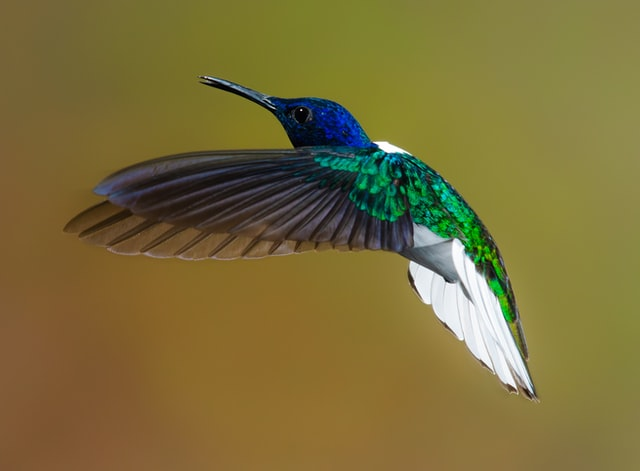
\includegraphics[width=\cellwidth]{img/bird.jpg}
            \end{cell}
            \begin{cell}{0.05}
                ~
            \end{cell}
            \begin{cell}{0.3}
                Lorem ipsum dolor sit amet, consectetur adipiscing elit. Vivamus eget mauris sed ligula blandit tristique. Quisque laoreet ac odio hendrerit pretium. Sed hendrerit id elit id lobortis. Aliquam ante eros, euismod et ultricies in, suscipit at lectus. Class aptent taciti sociosqu ad litora torquent per conubia nostra, per inceptos himenaeos. Cras eu massa congue justo egestas ornare pellentesque in quam.
            \end{cell}
        \end{row}
        \begin{row}{0.05}
            \begin{cell}{1}
                ~ 
            \end{cell}
        \end{row}
        \begin{row}{0.3}
            \begin{cell}{0.3}
                
\includegraphics[width=\cellwidth, height=\rowheight, keepaspectratio]{img/cat.jpg}
            \end{cell}
            \begin{cell}{0.05}
                ~
            \end{cell}
            \begin{cell}{0.3}
                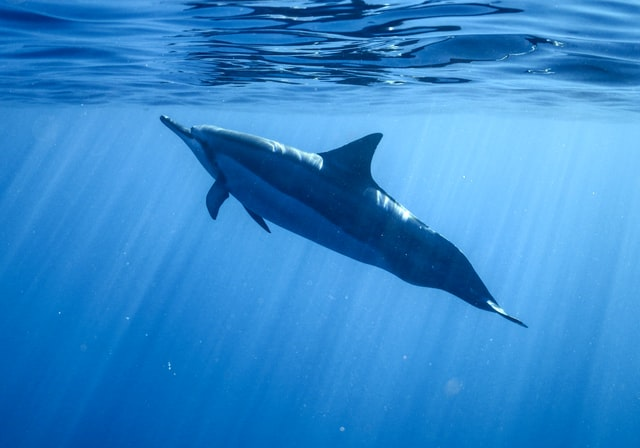
\includegraphics[width=\cellwidth, height=\rowheight, keepaspectratio]{img/dolphin.jpg}
            \end{cell}
            \begin{cell}{0.05}
                ~
            \end{cell}
            \begin{cell}{0.3}
                \centering
                \vspace{1em}
                \begin{tabular}{lr}
                    \toprule
                    Animal & Comment \\
                    \midrule
                    Bird & Colorful back \\
                    Cat & Cute look \\
                    Dolphin & Underwater \\
                    \bottomrule
                \end{tabular}
            \end{cell}
        \end{row}
    \end{gridlayout}
\end{example}


%%%%%%%%%%%%%%%%%%%%%%%%%%%%%%%% END OF CONTENT

\end{document}
